\chapter{Gráficos do Experimento 5 da Etapa 1}

As Figuras \ref{fig:graphCO-01}-\ref{fig:graphCO-10} apresentam a evolução do VPL da melhor solução, da pior solução e a média da população das dez execuções da segunda proposta de Algoritmo Genético de Regime Permannete com o contador de ocorrências durante o Experimento 5 da Etapa 1 ($AG^{CO-1}$) com a a população composta por 100 indivíduos.

\begin{figure}[H]
\centering

\includegraphics[scale=1]{apxE/agco1/1}
\caption{Evolução do VPL para a primeira execução da segunda versão modificada de Algoritmo de Regime Permanente com o contador de ocorrências a com 100 indivíduos na população.}
\label{fig:graphCO-01}
\end{figure}

\begin{figure}[H]
\centering

\includegraphics[scale=1]{apxE/agco1/2}
\caption{Evolução do VPL para a segunda execução da segunda versão modificada de Algoritmo de Regime Permanente com o contador de ocorrências a com 100 indivíduos na população.}
\label{fig:graphCO-02}
\end{figure}

\begin{figure}[H]
\centering

\includegraphics[scale=1]{apxE/agco1/3}
\caption{Evolução do VPL para a terceira execução da segunda versão modificada de Algoritmo de Regime Permanente com o contador de ocorrências a com 100 indivíduos na população.}
\label{fig:graphCO-03}
\end{figure}
\begin{figure}[H]
\centering

\includegraphics[scale=1]{apxE/agco1/4}
\caption{Evolução do VPL para a quarta execução da segunda versão modificada de Algoritmo de Regime Permanente com o contador de ocorrências a com 100 indivíduos na população.}
\label{fig:graphCO-04}
\end{figure}
\begin{figure}[H]
\centering

\includegraphics[scale=1]{apxE/agco1/5}
\caption{Evolução do VPL para a quinta execução da segunda versão modificada de Algoritmo de Regime Permanente com o contador de ocorrências a com 100 indivíduos na população.}
\label{fig:graphCO-05}
\end{figure}
\begin{figure}[H]
\centering

\includegraphics[scale=1]{apxE/agco1/6}
\caption{Evolução do VPL para a sexta execução da segunda versão modificada de Algoritmo de Regime Permanente com o contador de ocorrências a com 100 indivíduos na população.}
\label{fig:graphCO-06}
\end{figure}
\begin{figure}[H]
\centering

\includegraphics[scale=1]{apxE/agco1/7}
\caption{Evolução do VPL para a sétima execução da segunda versão modificada de Algoritmo de Regime Permanente com o contador de ocorrências a com 100 indivíduos na população.}
\label{fig:graphCO-07}
\end{figure}
\begin{figure}[H]
\centering

\includegraphics[scale=1]{apxE/agco1/8}
\caption{Evolução do VPL para a oitava execução da segunda versão modificada de Algoritmo de Regime Permanente com o contador de ocorrências a com 100 indivíduos na população.}
\label{fig:graphCO-08}
\end{figure}
\begin{figure}[H]
\centering

\includegraphics[scale=1]{apxE/agco1/9}
\caption{Evolução do VPL para a noba execução da segunda versão modificada de Algoritmo de Regime Permanente com o contador de ocorrências a com 100 indivíduos na população.}
\label{fig:graphCO-09}
\end{figure}
\begin{figure}[H]
\centering
\includegraphics[scale=1]{apxE/agco1/10}
\caption{Evolução do VPL para a décima execução da segunda versão modificada de Algoritmo de Regime Permanente com o contador de ocorrências a com 100 indivíduos na população.}
\label{fig:graphCO-10}
\end{figure}

As Figuras \ref{fig:graphCO-01}-\ref{fig:graphCO-10} apresentam a evolução do VPL da melhor solução, da pior solução e a média da população das dez execuções da segunda proposta de Algoritmo Genético de Regime Permannete com o contador de ocorrências durante o Experimento 5 da Etapa 1 ($AG^{CO-1}$) com a a população composta por 50 indivíduos.

\begin{figure}[H]
\centering
\includegraphics[scale=1]{apxE/agco2/1}
\caption{Evolução do VPL para a primeira execução da segunda versão modificada de Algoritmo de Regime Permanente com o contador de ocorrências a com 50 indivíduos na população.}
\label{fig:graphCO2-01}
\end{figure}

\begin{figure}[H]
\centering
\includegraphics[scale=1]{apxE/agco2/2}
\caption{Evolução do VPL para a segunda execução da segunda versão modificada de Algoritmo de Regime Permanente com o contador de ocorrências a com 50 indivíduos na população.}
\label{fig:graphCO2-02}
\end{figure}

\begin{figure}[H]
\centering
\includegraphics[scale=1]{apxE/agco2/3}
\caption{Evolução do VPL para a terceira execução da segunda versão modificada de Algoritmo de Regime Permanente com o contador de ocorrências a com 50 indivíduos na população.}
\label{fig:graphCO2-03}
\end{figure}

\begin{figure}[H]
\centering
\includegraphics[scale=1]{apxE/agco2/4}
\caption{Evolução do VPL para a quarta execução da segunda versão modificada de Algoritmo de Regime Permanente com o contador de ocorrências a com 50 indivíduos na população.}
\label{fig:graphCO2-04}
\end{figure}

\begin{figure}[H]
\centering
\includegraphics[scale=1]{apxE/agco2/5}
\caption{Evolução do VPL para a quinta execução da segunda versão modificada de Algoritmo de Regime Permanente com o contador de ocorrências a com 50 indivíduos na população.}
\label{fig:graphCO2-05}
\end{figure}

\begin{figure}[H]
\centering
\includegraphics[scale=1]{apxE/agco2/6}
\caption{Evolução do VPL para a sexta execução da segunda versão modificada de Algoritmo de Regime Permanente com o contador de ocorrências a com 50 indivíduos na população.}
\label{fig:graphCO2-06}
\end{figure}

\begin{figure}[H]
\centering
\includegraphics[scale=1]{apxE/agco2/7}
\caption{Evolução do VPL para a sétima execução da segunda versão modificada de Algoritmo de Regime Permanente com o contador de ocorrências a com 50 indivíduos na população.}
\label{fig:graphCO2-07}
\end{figure}

\begin{figure}[H]
\centering
\includegraphics[scale=1]{apxE/agco2/8}
\caption{Evolução do VPL para a oitava execução da segunda versão modificada de Algoritmo de Regime Permanente com o contador de ocorrências a com 50 indivíduos na população.}
\label{fig:graphCO2-08}
\end{figure}

\begin{figure}[H]
\centering
\includegraphics[scale=1]{apxE/agco2/9}
\caption{Evolução do VPL para a nona execução da segunda versão modificada de Algoritmo de Regime Permanente com o contador de ocorrências a com 50 indivíduos na população.}
\label{fig:graphCO2-09}
\end{figure}

\begin{figure}[H]
\centering
\includegraphics[scale=1]{apxE/agco2/10}
\caption{Evolução do VPL para a décima execução da segunda versão modificada de Algoritmo de Regime Permanente com o contador de ocorrências a com 50 indivíduos na população.}
\label{fig:graphCO2-10}
\end{figure}